\section{Assignment 3: Scale-Invariant Blob Detection}
\label{sec:assignment3}

This assignment is about locating blobs of different sizes in images. A Laplacian blob detector is implemented and used in a scale-invariant way by convolving it with repeatedly blurred versions of the image to be analysed.
Interest point detectors in general are discussed in \cite{Szeliski}, and LoG as a feasible scale invariant detector in \cite{Lindeberg} and \cite{Mikolajczyk}.

\subsection{Problem definition}

Given an image, the problem is to find blob-like features of varying scale. In specific, the goals are to:
\begin{itemize}[noitemsep]
\item Implement a Laplacian of Gaussian (LoG) blob detector
\item Apply it to a reference image (\texttt{butterfly.jpg}) and an image of choice, and to also apply it to half-sized versions of the images
\item Indicate the found blobs by overlaying circles, with the circle radii being representative of the found blob's size
\item Plot the LoG response over all scales at a specific key point for both the original and half-sized image
\item Discuss the results
\end{itemize}

\subsection{Methodology}
\label{sec:a3:methodology}

The detector parameters and image filename (\texttt{sigma0, k, level, thresh, FILENAME}) are defined in the first couple of lines of the implementation and can easily be changed there to experiment with different values.
After loading the image, we create a scale space matrix of depth \texttt{level}, each level corresponding to a specific value of $\sigma$.
The original image is convoluted with an LoG-filter of size proportional to increasing values of $\sigma$ ($= \sigma_0 k^{level-1}$), and the result is stored in the scale-space-matrix, so that each level represents the filter response to an increasingly blurred version of the image.
In order to detect blobs independently of the intensity relative to their background, we store the absolute value of the filter response.

Non-maxima-suppression is then performed on the scale-space-matrix, leaving only those elements non-zero, which are larger than all of their 26 immediate neighbours in the three-dimensional matrix. Each of these remaining points corresponds to the centre of a detected blob (dimension 1 and 2 of the matrix), and the blob's size (dimension 3: $\sigma$).

\subsection{Experiments}

We experimented with two images (\texttt{butterfly.jpg} and \texttt{dalmation.png}) and used the blob detector on both the original as well as a half-sized version of each. Figure \ref{fig:a3:general} demonstrates the results for a specific set of parameters ($\sigma_0=2, k=1.25, threshold=0.20, levels=10$). It can be seen, that the detector finds most blobs in a scale-invariant way; specifically matching blobs are found in both scalings of an image, if both their original radius and half sized radius are in the range covered by parameters $\sigma, k, levels$: the size of detected blobs is limited by the range of $\sigma$-values; only blobs whose radius lies in $r_{min} \leq r \leq r_{max}$ ($r_{min} = \sigma_0 \sqrt{2}$ and $r_{max} = \sigma_0 k^{levels-1}  \sqrt{2}$) will be found. Scale invariance can break in one of three ways: Either a blob is too large to be found in the original image, but small enough so that its half-sized appearance in the half-sized image is detected (e.g. the large blob at the right wing tip of the butterfly in Figure \ref{fig:a3:general}, bottom right image); or it is too small to be found in the half-sized image, but large enough to be detected in the original (e.g., the small blobs on the hind paw of the Dalmatian in Figure \ref{fig:a3:general}, top left image). A third possible way, which we did not observe, could arise if the downscaling process of the image alters the intensity values in such a way, that a potential blob is excluded from one image during non-maxima-suppression (due to thresholding), but not in the other.

\begin{figure}[h]
	\centering
	\begin{tabular}{cc}
		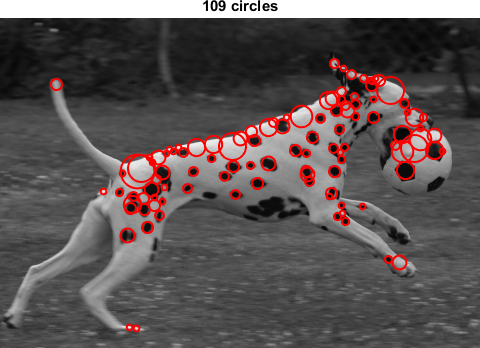
\includegraphics[width=0.5\textwidth]{figures/a3_dalmation_k020_full.png} &
		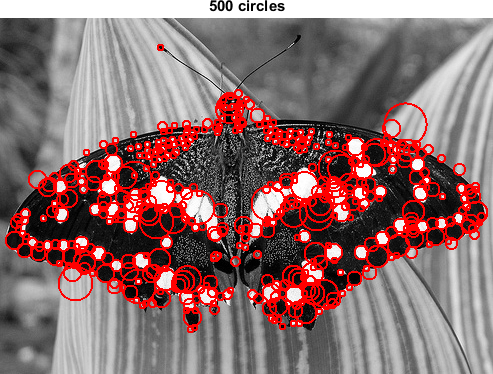
\includegraphics[width=0.5\textwidth]{figures/a3_butterfly_k020.png} \\
		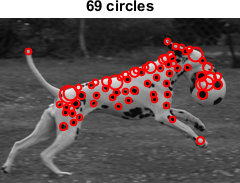
\includegraphics[width=0.25\textwidth]{figures/a3_dalmation_k020_half.png} &
		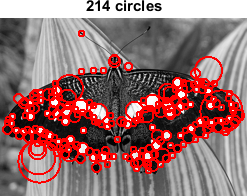
\includegraphics[width=0.25\textwidth]{figures/a3_butterfly_k020_small.png} \\
	\end{tabular}
	\caption{LoG blob detector applied to two different images and to half-sized versions of them. Parameters: $\sigma_0=2, k=1.25, threshold=0.20, levels=10$.}
	\label{fig:a3:general}
\end{figure}

We experimented with different threshold values to find satisfactory values; see Figure \ref{fig:a3:thresholds} for results. Obviously, the lower the threshold is, the more blobs are found. Our final choice of $threshold=0.20$ was obtained by a subjective judgement, i.e. if we considered the results to be ``real'' blobs or not. This leads to ambiguities though; for example, we would consider the blotches in the bottom left background (Figure \ref{fig:a3:thresholds}, top left image) to be more ``real'' blobs than the leaf segment above the right wing; however with increasing threshold the blotches disappear first, while the leaf segments persist.

\begin{figure}[h]
	\centering
	\begin{tabular}{cc}
	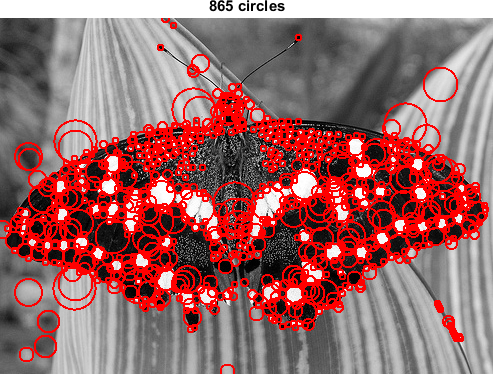
\includegraphics[width=0.5\textwidth]{figures/a3_butterfly_k015.png} &
	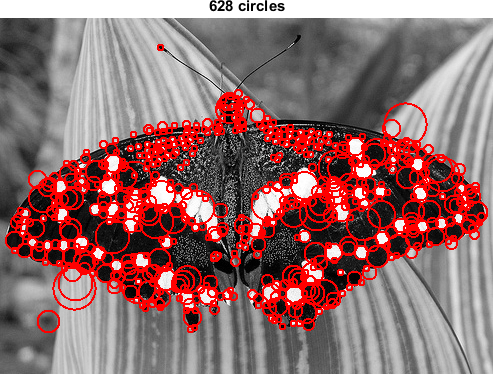
\includegraphics[width=0.5\textwidth]{figures/a3_butterfly_k018.png} \\
	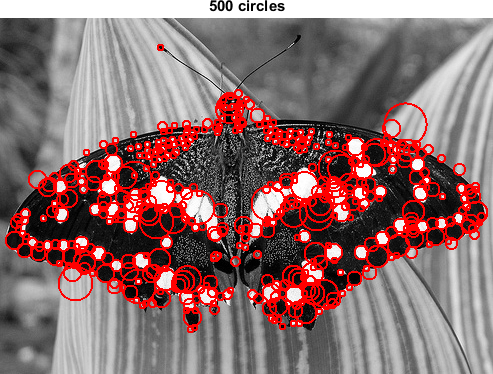
\includegraphics[width=0.5\textwidth]{figures/a3_butterfly_k020.png} &
	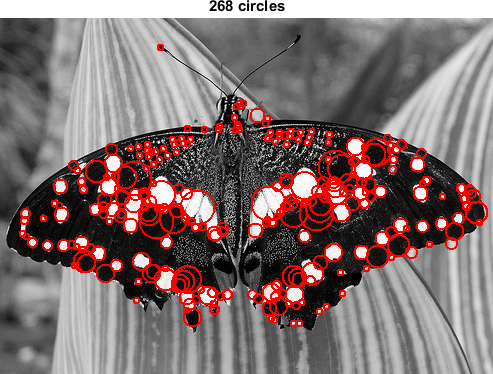
\includegraphics[width=0.5\textwidth]{figures/a3_butterfly_k025.png} \\
	\end{tabular}
	\caption{Illustration of the effect of different thresholds $t$. Top left: $t=0.15$. Top right: $t=0.18$. Bottom left: $t=0.20$. Bottom right: $t=0.25$.}
	\label{fig:a3:thresholds}
\end{figure}

Additionally, we examined the LoG response over all scale levels for specific key points (blob centres). Figure \ref{fig:a3:logresponse} shows the response for two distinct key points of the butterfly image. When comparing the responses of the original image to those of the half-sized version, it can be seen that the extremal values appear on different scale levels. E.g., for the key point on the left side of Figure \ref{fig:a3:logresponse}, we find the extrema (minima in this case) at level 9 ($\sigma_{full}=11.92$) for the full resolution and level 6 ($\sigma_{half}=6.10$) for the half-sized blob respectively. Indeed $\sigma_{full} : \sigma_{half} \approx 2:1$ as expected, i.e. the radius in the full image is twice as large.

It can also be seen that the initial LoG response is sensitive to the gradient direction. E.g., a bright blob on dark background produces a minimal response at the correct scale, while a dark blob on bright background produces a maximal response. Since we do not care about the gradient direction to detect blobs, we only search for maxima of the \textit{absolute} response, as described in Section \ref{sec:a3:methodology}.

\begin{figure}[h]
	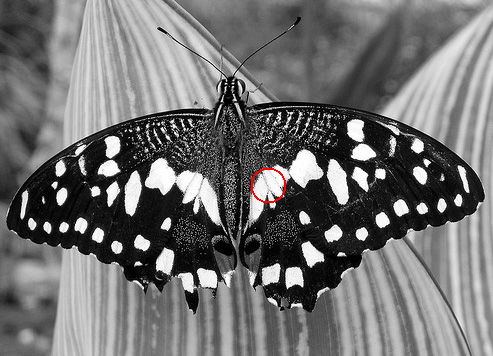
\includegraphics[width=0.5\textwidth]{figures/a3_butterfly_keypoint.png}
	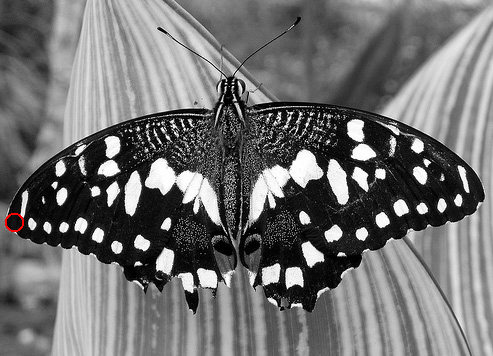
\includegraphics[width=0.5\textwidth]{figures/a3_butterfly_keypoint_2.png}
	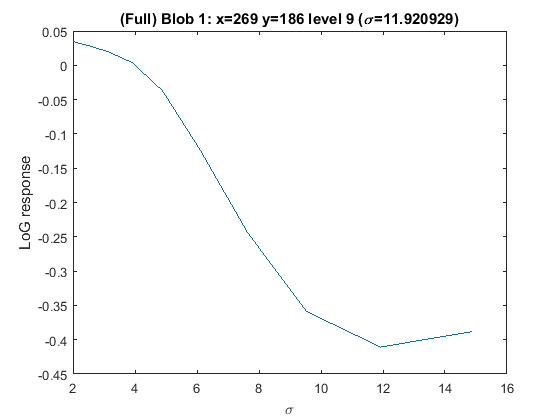
\includegraphics[width=0.5\textwidth]{figures/a3_butterfly_log_full.png}
	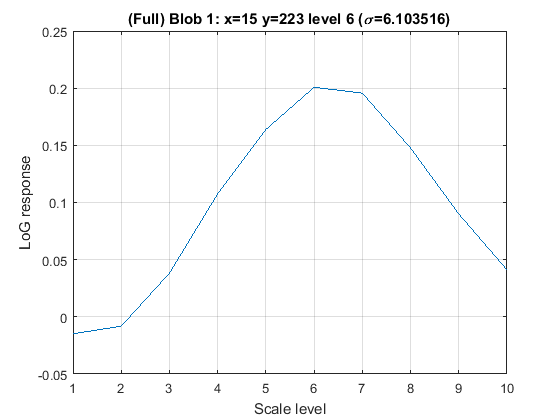
\includegraphics[width=0.5\textwidth]{figures/a3_butterfly_log_full_2.png}
	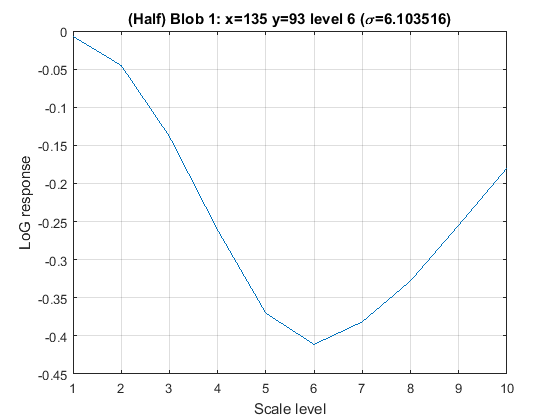
\includegraphics[width=0.5\textwidth]{figures/a3_butterfly_log_half.png}
	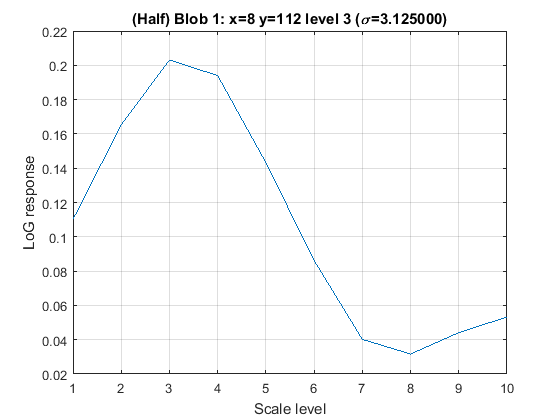
\includegraphics[width=0.5\textwidth]{figures/a3_butterfly_log_half_2.png}
	\caption{LoG response for two selected key points. The top row shows the chosen key point, the second and third rows show the LoG response for the full-sized and half-sized image. Left: A white-on-black blob (negative LoG response), right: a black-on-white blob (positive LoG response).}
	\label{fig:a3:logresponse}
\end{figure}

